\documentclass[../proyecto.tex]{subfiles}

\begin{document}
\chapter{Análisis del problema}\label{chap:analisis_del_problema}

En este capítulo se realizará un análisis del problema comenzando con una descripción de los requisitos que debe cumplir el sistema (\autoref{sect:analisis_requisitos}) para más tarde analizar las posibles soluciones que nos permitan cumplir los requisitos analizados anteriormente (\autoref{sect:analisis_soluciones}), culminando con la presentación de la solución elegida. Para ayudar a la organización de este capítulo cada una de estas secciones se ha divido a su vez en dos subsecciones, una para el análisis del sensor y otra para el análisis del servidor central.\\

\section{Análisis de requisitos}\label{sect:analisis_requisitos}

\subsection{Sensor}

\noindent{\textbf{Requisitos funcionales}}
\begin{itemize}
  \item El sensor será capaz de detectar y registrar dispositivos BLE (Bluetooth Low Energy) cercanos.
  \item El sensor será capaz de detectar y registrar dispositivos WiFi cercanos.
  \item El sensor realizará el envío de las detecciones realizadas mediante el protocolo HTTP a través de una conexión WiFi.
\end{itemize}

\noindent{\textbf{Requisitos no funcionales}}
\begin{itemize}
  \item Bajo coste (< 15€).
  \item Bajo consumo energético (< 250 mA).
  \item Reducidas dimensiones (< 80 x 50 mm)
\end{itemize}


\subsection{Servidor Central}

\noindent{\textbf{Requisitos funcionales}}
\begin{itemize}
  \item El sistema dispondrá de una API REST que permitirá crear, listar, modificar y eliminar tanto detecciones como sensores.
  \item El sistema dispondrá de una interfaz web que permitirá visualizar las detecciones realizadas y la información de los sensores en forma de tablas.
\end{itemize}

\noindent{\textbf{Requisitos no funcionales}}
\begin{itemize}
  \item El frontal web debe poder visualizarse correctamente en los principales navegadores (Chrome, Firefox e Internet Explorer).
  \item El frontal web debe adaptarse a diferentes resoluciones de pantalla.
  \item El sistema permitirá su despliegue sobre contenedores.
\end{itemize}

\noindent{\textbf{Requisitos de información}}

\begin{itemize}
  \item Se almacenarán de forma persistente los datos de las detecciones enviadas al sistema (identificador, dirección MAC, fecha y hora e identificador del sensor que ha realizado la detección).
  \item Se almacenarán de forma persistente los datos de los sensores conectados al sistema (identificador y descripción).
\end{itemize}


\section{Análisis de las soluciones}\label{sect:analisis_soluciones}
En esta sección se realizará un análisis de las tecnologías y herramientas que han sido necesarias para cumplir los objetivos de este proyecto. Se diferenciaran dos secciones, en la primera se agruparán las tecnologías relacionadas con el sensor y en la segunda las relacionadas con el servidor central.\\

En cada subsección se presentará un resumen de los requisitos que se buscaban en cada tecnología, un repaso de las soluciones disponibles en el mercado y finalmente la solución seleccionada junto a la motivación para su elección.\\


\subsection{Sensor}
\subsubsection{SoC}
Los principales requisitos que debe cumplir la plataforma elegida son:

\begin{itemize}
  \item Conectividad WiFi y Bluetooth.
  \item Bajo coste (< 15€).
  \item Bajo consumo energético (<250 mA).
  \item Reducidas dimensiones.
\end{itemize}

Además de estos requisitos se definen otros aspectos no indispensables pero deseables:

\begin{itemize}
  \item Facilidad de programación.
  \item Madurez en el mercado.
  \item Buena documentación.
  \item Gran comunidad de usuarios.
\end{itemize}

\paragraph{Arduino}\mbox{}\\

Una de las primeras plataformas analizadas fue Arduino por su gran popularidad, estas placas empezaron su andadura en el 2005 y han cosechado una gran comunidad, pero hasta hace relativamente poco no ofrecían soluciones con conectividad WiFi y Bluetooth integrada si no que se basaban en el uso de módulos de expansión (\textit{shields}) para dotar a sus placas de conectividad inalámbrica lo cual encarecía el coste final, pero en 2018 decidieron cambiar con la placa Arduino MKR WiFi 1010 \cite{arduino_mkr_wifi_1010}, utiliza el SoC ESP32 fabricado por U-BLOX y dispone de conectividad WiFi y Bluetooth integrada en un empaquetado de solo 61.5x25 mm, más tarde en 2019 lanzaron el modelo Arduino Nano 33 IOT \cite{arduino_nano_33_iot} (Figura \ref{fig:arduino_nano_33_iot}) con prácticamente las mismas características y algunas mejoras como la inclusión de un acelerómetro pero sacrificando el conector de batería y la compatibilidad con los \textit{shields} en favor de un menor tamaño (48 × 18 mm) y menor coste. Esta última solución encajaba con la mayoría de los requisitos excepto con el coste, tiene un precio de aproximadamente 25€ que queda muy por encima del objetivo de coste, además su poca madurez en el mercado juega también en su contra.

\begin{figure}[H]
\centering
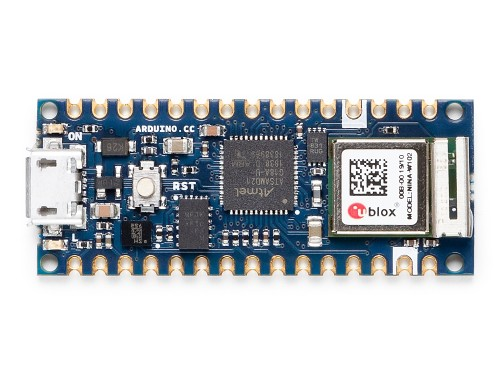
\includegraphics[scale=0.45]{analisis/arduino_nano_33_iot}
\caption{Arduino Nano 33 IOT}
\label{fig:arduino_nano_33_iot}
\end{figure}

\paragraph{Espressif Systems SoCs}\mbox{}\\

Espressif es una compañía fundada en 2008 en China y con sede en Shanghai enfocada en el desarrollo de soluciones IoT que desarrolla \textit{chipsets} y módulos WiFi y/o Bluetooth/BLE de pequeñas dimensiones con un gran rendimiento, bajo consumo y coste enfocados principalmente a dotar de conectividad a los productos de otras compañías. Son los creadores de los populares SoCs ESP8266 y ESP32 que además tener una gran penetración en el mercado de IoT han tenido un gran éxito en la comunidad \textit{maker}.\\

\noindent{\textbf{ESP8266}}

El ESP8266, oficialmente ESP8266EX, es un SoC WiFi de bajo coste con una pila TCP/IP lanzado al mercado en 2014 \cite{esp8266_overview}, este fue el módulo con el que Espressif comenzó a popularizarse. Se comercializa principalmente en tres formatos: SoC, módulos y módulos de desarrollo (\textit{DevKit}). Espressif desarrollo este SoC pensando en las necesidades de la industria del Internet of Things, como son el bajo consumo energético, un diseño compacto y la fiabilidad y durabilidad. Con una capacidad WiFi completa y autónoma puede funcionar de forma independiente o como adaptador WiFi para cualquier controlador a través de las interfaces SPI/SDIO o UART. Estas cualidades han propiciado que su utilización se haya extendido en la industria de la domótica, por ejemplo, en enchufes y bombillas inteligentes. \\

Integra un microcontrolador Tensilica L106 de 32 bits (RISC) de bajo consumo que trabaja a unos 80 MHz por defecto pudiendo alcanzar hasta 160 MHz. Además incorpora otros componentes de interfaz como SDIO, SPI, I2C, I2S, UART, PWM, conversor ADC de 10 bits y 17 GPIO. Todos estos componentes se encuentran empaquetados en tan solo 5 mm x 5 mm en un formato QFN de 32 pines. En el SoC no viene incluida la memoria ROM, debe utilizarse una flash externa por SPI y soporta hasta 16 MB \cite{esp8266_datasheet}. Uno de sus principales atractivos es el precio, se pueden adquirir por menos de 1€ en los distribuidores oficiales de Espressif \cite{espressif_provider_digikey} \cite{espressif_provider_mouser}\\

Debido a que el ESP8266 viene en un pequeño empaquetado (QFN-21) algunos fabricantes han desarrollado módulos (MCU) que facilitan su uso, proporcionando componentes necesarios para el desarrollo como son la memoria flash externa y pines externos para GPIO.\\

\begin{table}[H]
\centering
\begin{tabular}{ |l|m{20em}| }
\hline
Voltaje de operación      & 2.5V $\sim$ 3.6V          \\ \hline
Consumo                   & 20 uA - 170 mA (80 mA avg.)  \\ \hline
Temperatura de operación  & -40°C $\sim$ 125°C        \\ \hline
Procesador                & Tensilica L106 32-bit     \\ \hline
Frecuencia de reloj       & 80 MHz / 160 MHz          \\ \hline
Interfaces                & UART, SDIO, SPI, I2C, I2S, IR Remote Control, GPIO, ADC y PWM                           \\ \hline
GPIO pins                 & 17                        \\ \hline
RAM (espacio de usuario)  & < 50 kB                     \\ \hline
Protocolos WiFi           & 802.11 b/g/n (HT20)       \\ \hline
Rango de frecuencias WiFi & 2.4G $\sim$ 2.5G (2400M $\sim$ 2483.5M) \\ \hline
\end{tabular}
\caption{Características ESP8266}
\label{table:caracteristicas_esp8266}
\end{table}

Espressif dispone de sus propio módulos, la serie ESP-WROOM-02 \cite{espwroom02_overview}, el módulo base \cite{espwroom02_datasheet} lleva el mismo nombre que la serie y tiene un tamaño de 18 mm x 20 mm e integran una memoria flash SPI de 2 MB y una antena PCB, además dispone de 18 pines. Existen otros modelos de la serie con 4MB de memoria flash y con conectores IPEX para una antena externa en lugar de la antena PCB. El precio medio de esta serie es de 2,50€ \cite{espressif_provider_digikey} \cite{espressif_provider_mouser}.\\

A pesar de que el fabricante original del ESP8266, Espressif, dispone de sus propios módulos, este SoC empezó realmente a popularizarse en 2014 con el módulo ESP-01 creado por un tercer fabricante, Ai-Thinker. El módulo añade una memoria flash externa QSPI, una antena impresa en la PCB y proporciona salida para algunos de los pines del ESP8266. Desde este primer modelo se han desarrollado multitud de modelos con variaciones respecto al número de pines expuestos, tipo de antena y memoria flash; pero manteniendo el mismo SoC ESP8266EX. Se les conoce como módulos ESP-XX, el modelo más utilizado de esta serie es el ESP-12 (Figura \ref{fig:esp12}). \\

\begin{figure}[H]
\centering
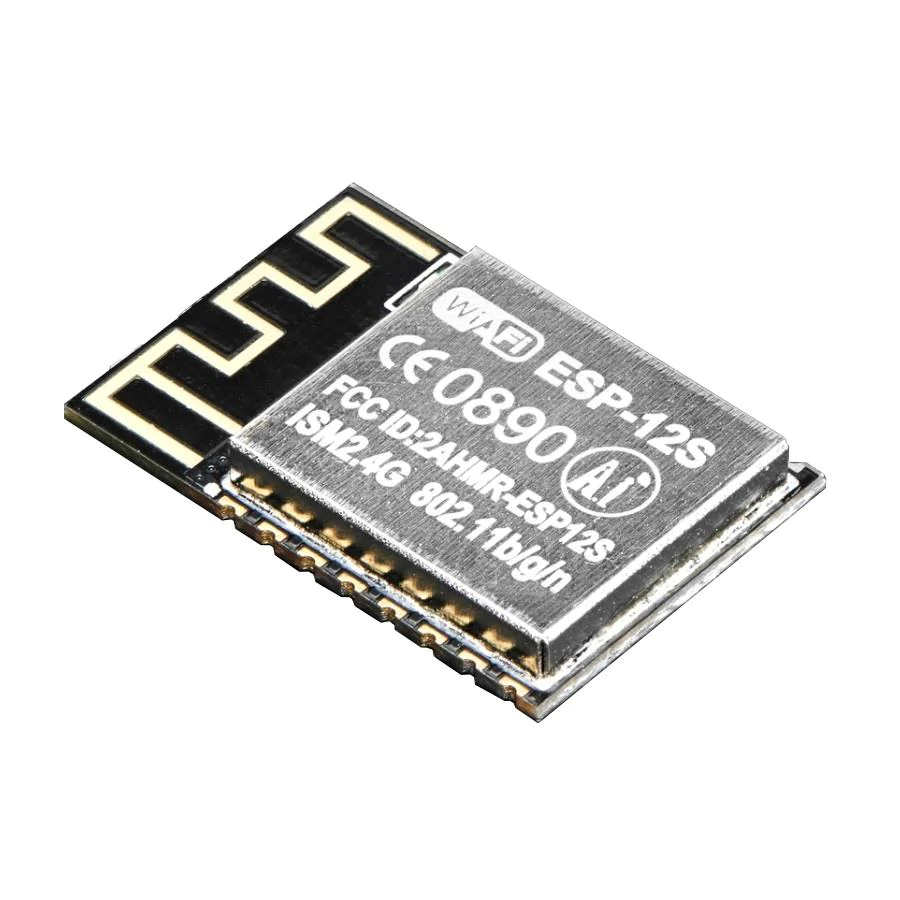
\includegraphics[scale=0.12]{analisis/esp12}
\caption{Módulo ESP-12S}
\label{fig:esp12}
\end{figure}

\newpage

Aunque estos módulos son más cómodos seguimos teniendo la necesidad de adquirir un adaptador USB-Serial, un regulador de voltaje y cablearlos al módulo para poder programarlo y alimentarlo. Para suplir estas necesidades nacieron los módulos de desarrollo (Devkits), estos módulos están enfocados al desarrollo rápido y a facilitar la creación de prototipos, para ello incluyen un puente USB-Serial integrado en la placa y un conector micro-USB junto con un regulador de voltaje para proporcionar energía a la placa y conectividad con el ordenador, además de otras facilidades como botones, leds o conectores para baterías y antenas.\\

Algunos modelos están basado en módulos ESP-XX de Ai-Thinker como el Adafruit Feather HUZZAH \cite{adafruit_feather_huzzah} que utiliza un módulo Ai-Thinker ESP-12S, en la figura \ref{fig:adafruit_feather_huzzah_pinout_2} se pude apreciar como el módulo de Ai-thinker está soldado directamente encima de la placa de desarrollo.\\~\\

\begin{figure}[H]
\centering
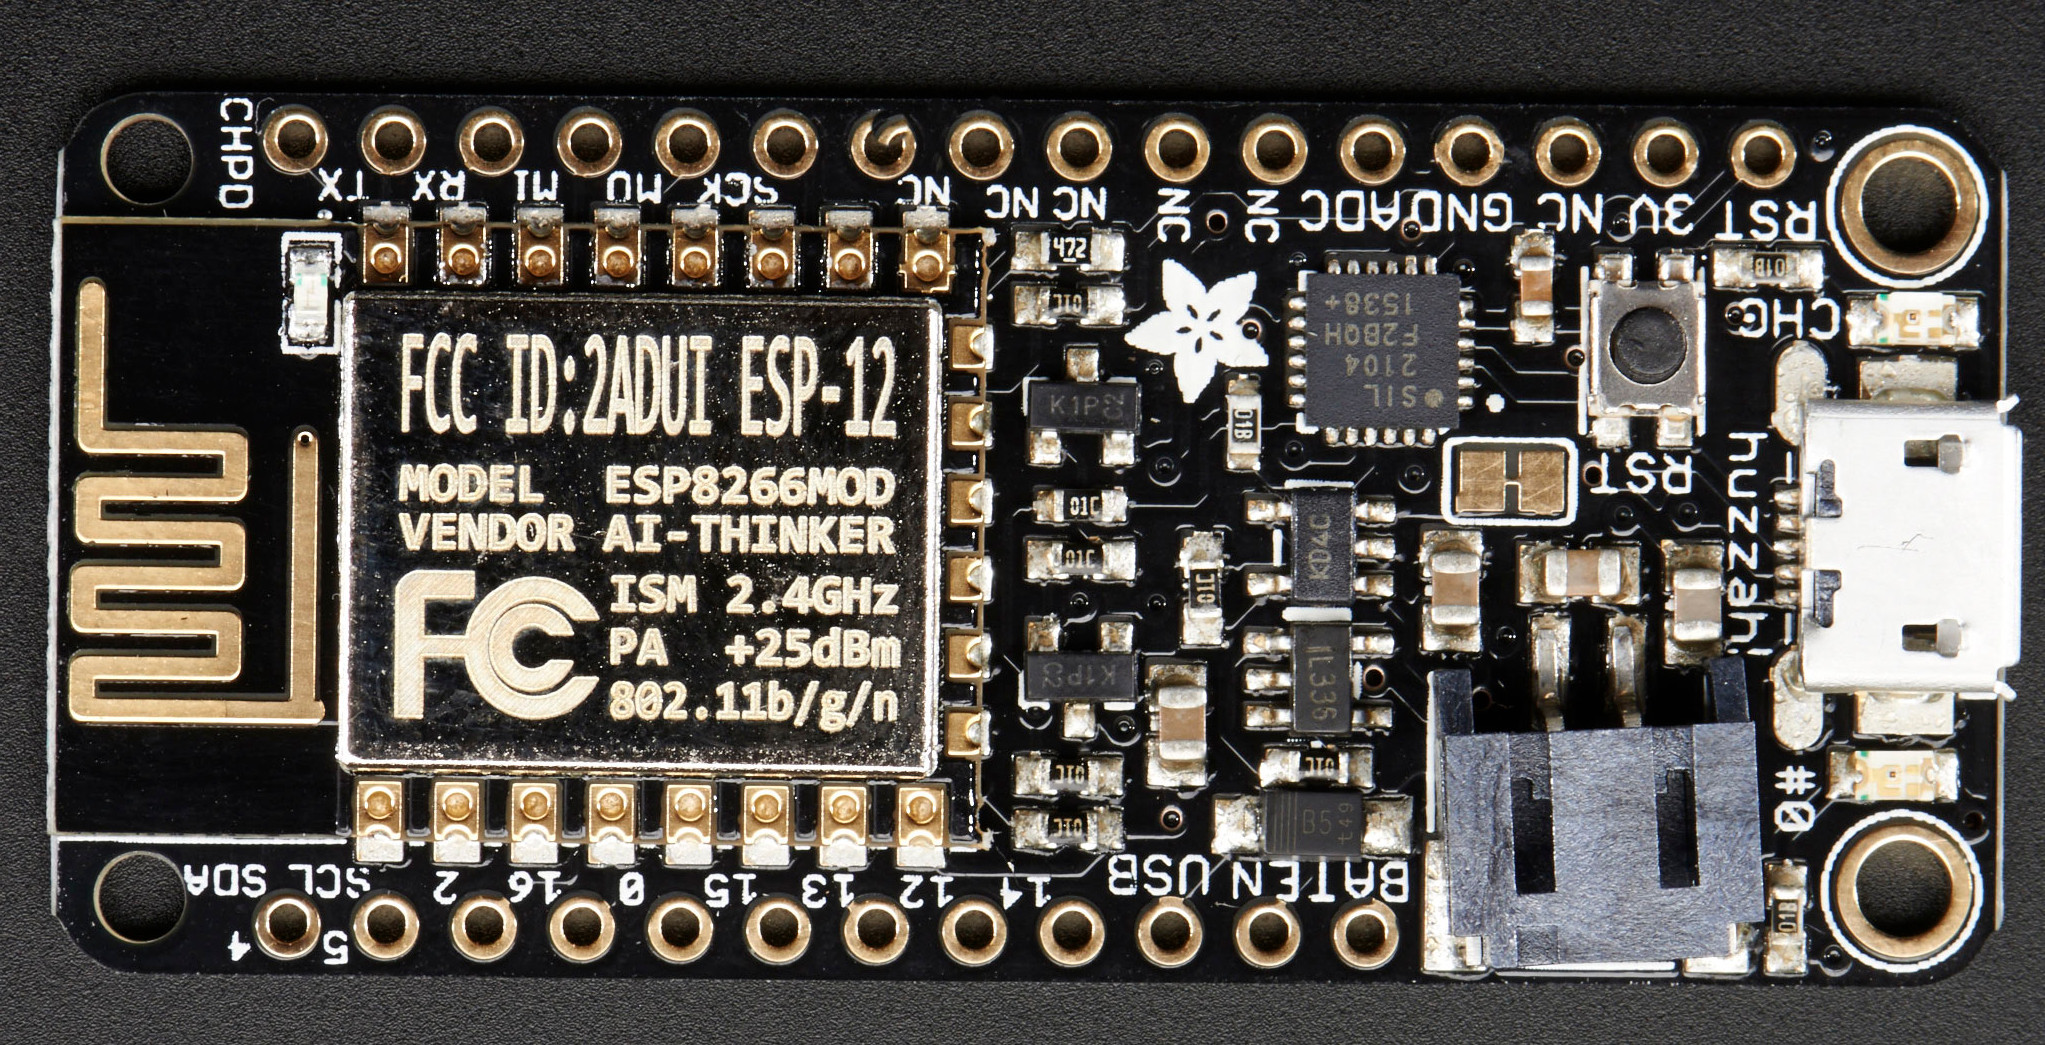
\includegraphics[scale=0.10]{analisis/adafruit_feather_huzzah_pinout_2}
\caption{Adafruit Feather HUZZAH}
\label{fig:adafruit_feather_huzzah_pinout_2}
\end{figure}

Otros módulos de desarrollo no usan un módulo intermediario, en su lugar incorporan directamente el SoC en la placa como es el caso del WEMOS D1 Mini Pro \cite{wemos_d1_mini_pro} que utiliza un ESP8266EX (Figura \ref{fig:wemos_d1_mini_pro}).\\

\begin{figure}[h]
\centering
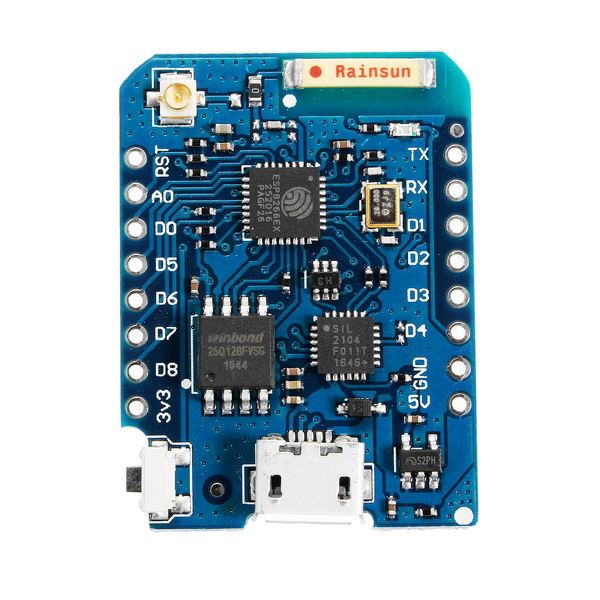
\includegraphics[scale=0.3]{analisis/wemos_d1_mini_pro}
\caption{WEMOS D1 Mini Pro}
\label{fig:wemos_d1_mini_pro}
%https://wiki.wemos.cc/products:retired:d1_mini_pro_v1.1.0
\end{figure}

Existen una gran variedad de estos módulos de diferentes fabricantes, algunos de los más conocidos son:  Feather de la empresa Adafruit Industries, ESP8266 Thing de la empresa SparkFun Electronics y NodeMCU del fabricante Lolin. Hay un gran rango de precios desde los 3€ del modelo de WEMOS a los 15€ del modelo de SparkFun \cite{espressif_provider_digikey} \cite{espressif_provider_mouser}\cite{sparkfun_thing_official_page}.\\

\noindent{\textbf{ESP32}}\\

El ESP32, es una familia de SoC's de bajo coste y consumo con WiFi y Bluetooth modo dual integrado, también diseñado por Espressif Systems \cite{esp32_overview} es el sucesor del ESP8266.\\

La familia de SoCs ESP32 dispone de una gran variedad de modelos la mayoría en un formato QFN de 5x5 mm y 6x6 mm a excepción de la familia PICO que usan un encapsulado LGA de 7x7 mm, todos los modelos tienen 48 pines y utilizan microprocesadores Xtensa 32-bit LX6 en versiones de un solo núcleo o dos dependiendo del modelo, ambas versiones pueden trabajar en frecuencias desde 80 MHz hasta 240MHz. Al desarrollar estos nuevos SoCs Espressif les dotó de características ideales para dispositivos \textit{wearables} como el soporte para BLE, sensores táctiles capacitivos o modo de sueño para ahorro energético con el que consume menos de 5  uA. El precio de estos SoCs oscila entre 0,89€ y 3€ en los distribuidores oficiales de Espressif \cite{espressif_provider_digikey} \cite{espressif_provider_mouser}.\\

\begin{table}[H]
\centering
\begin{tabular}{ |l|m{20em}| }
\hline
Voltaje de operación      & 2.3V $\sim$ 3.6V          \\ \hline
Consumo                   & 10 uA - 68 mA  \\ \hline
Temperatura de operación  & -40°C $\sim$ 125°C        \\ \hline
Procesador                & Xtensa single-/dual-core 32-bit LX6 microprocessor(s)   \\ \hline
Frecuencia de reloj       & 80 MHz / 160 MHz  / 240 MHz        \\ \hline
Interfaces                & 3 x UART, SDIO, 4 x SPI, 2 x I2C, 2 x I2S, IR, 12-bit SAR ADC, 2 x 8-bit DAC, CAN 2.0, 10 x touch sensors, SD card interface, Ethernet y PWM                           \\ \hline
GPIO pins                 & 34                        \\ \hline
RAM (espacio de usuario)  & < 50 kB                     \\ \hline
Protocolos WiFi           & 802.11 b/g/n (HT20)       \\ \hline
Rango de frecuencias WiFi & 2.4G $\sim$ 2.5G (2400M $\sim$ 2483.5M) \\ \hline
Bluetooth           &  Bluetooth v4.2 BR/EDR y BLE dual-mode  \\ \hline
\end{tabular}
\caption{Características ESP32}
\label{table:caracteristicas_esp32}
\end{table}

Al igual que su predecesor se comercializa en tres formatos: SoC, módulos y \textit{DevKits}. Esta vez Espressif apostó desde el principio por comercializar sus propios módulos y desarrolló una gran variedad de módulos, actualmente comercializa 13 variantes agrupadas en tres familias: ESP32-SOLO, ESP32-WROOM y ESP32-WROVER \cite{espressif_products_ordering_information}. La familia SOLO integra SoCs de un solo núcleo mientras las familias WROOM y WROVER utilizan doble núcleo, además esta última tiene memoria SPIRAM ideal para aplicaciones que requieren más memoria como productos AIoT. Con unas dimensiones que van desde los 18.00×25.50×3.10 mm hasta los 18.00×31.40×3.30 mm estos módulos contienen una memoria flash (4, 8 y 16 MB) y antena impresa PCB o conector IPEX para poder conectar antenas de mayor potencia. El precio de estos módulos oscila entre los 1,80€ hasta los 4,50€ dependiendo del modelo \cite{espressif_provider_digikey} \cite{espressif_provider_mouser}.\\

\begin{figure}[H]
\centering
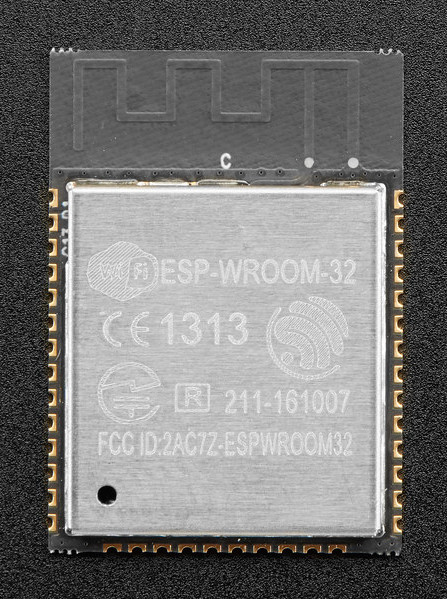
\includegraphics[scale=0.2]{analisis/esp32_module}
\caption{Módulo ESP32  \cite{esp32_module}.}
\label{fig:esp32_module}
\end{figure}

Espressif también ofrece una gran variedad de \textit{DevKits} para todo tipo de aplicaciones, desde placas con pantalla táctil integrada como la ESP32-S2-Kaluga-1, la ESP-EYE con cámara integrada para reconocimiento de imágenes e incluso placas con micrófonos, tecnologías de cancelación de ruido incorporadas y soporte para conectar con los servicios de asistente de voz de Google y Amazon como las ESP32-LyraTD. El modelo más básico, ESP32-DevKitC, se puede adquirir por aproximadamente 9€ en los distribuidores oficiales \cite{espressif_provider_digikey} \cite{espressif_provider_mouser}.\\

\paragraph{Elección}\mbox{}\\

Para el desarrollo de este proyecto se han utilizado módulos de desarrollo ya que facilitan un desarrollo rápido y cómodo al permitir programar y alimentar el módulo fácilmente a través de una conexión USB, aunque no es habitual utilizar este tipo de módulos en aplicaciones reales ya que encarecen el coste del despliegue al incluir componentes que no serían necesarios una vez desplegados como el adaptador USB-Serial, por otra parte nos permiten ahorrar en el diseño de la placa de alimentación y otros componentes.\\

Para el desarrollo de este proyecto en un principio se eligió el módulo de desarrollo WEMOS D1 Mini Pro basado en el SoC ESP8266, con unas dimensiones de 34.2 mm x 25.6 mm y un peso de 3 g es una de las placas más pequeñas del mercado, con un tamaño ligeramente más grande que un módulo ESP-12 (24.0 mm × 16.0 mm) incorpora un conversor P2104 USB-TO-UART, antena cerámica incorporada memoria flash de 16 MB y un regulador de tensión permite alimentarlo a 5 V a través de un micro-USB. Uno de los principales motivos para la elección de este módulo de desarrollo fue su reducido tamaño, la posibilidad de conectar una antena externa para mejorar el alcance mediante un conector de tipo U.FL y su reducido precio de tan solo 3€ \cite{lolin_official_store}. Otra de las ventajas de este módulo de desarrollo, a pesar de estar fuera del alcance de este proyecto, es la posibilidad de ampliar la funcionalidad a través de la conexión de expansiones en formato \textit{shields}. Existe una gran variedad \textit{shields} como, por ejemplo, pantalla oled, relé o controlador de motores.\\

Como punto negativo este módulo no cuenta con Bluetooth integrado por lo que para cumplir los requisitos de este proyecto es necesario usarlo junto a un módulo Bluetooth externo como el HC-05 (Figura \ref{fig:hc05_bluetooth_module}), estos módulos pueden conectarse con el ESP8266 usando el puerto serie y se configuran utilizando comandos AT, se pueden adquirir por alrededor de 2€ por lo que el coste total en componentes sería de aproximadamente unos 5€ por lo que seguiría cumpliendo el requisito del bajo coste.

\begin{figure}[H]
\centering
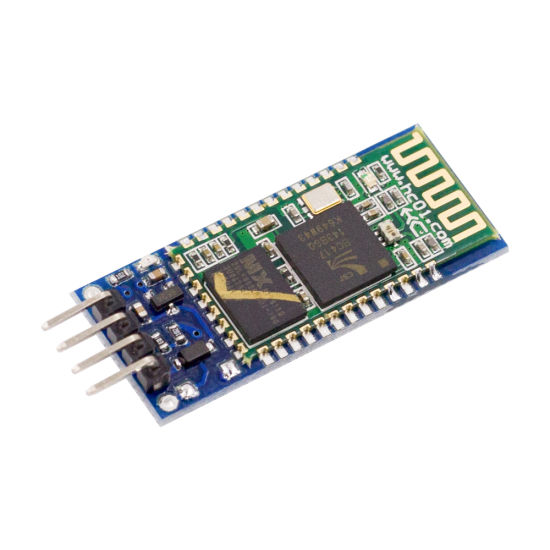
\includegraphics[scale=0.2]{analisis/hc05_bluetooth_module}
\caption{Módulo Bluetooth HC-05}
\label{fig:hc05_bluetooth_module}
\end{figure}

Por las razones expuestas inicialmente se decidió utilizar el SoC ESP8266 junto con el módulo Bluetooth HC-05 ya que cumplía con el requisito del bajo coste mejor que ninguna de las opciones incluso teniendo en cuenta el hecho de tener que adquirir el módulo Bluetooth por separado, pero durante el desarrollo del proyecto se apreció que en la valoración inicial no se había tenido en cuenta el coste que supondría el proceso de integración de estos módulo, aunque aparentemente una operación sencilla como es el soldado o cableado de estos dos módulos supondría un gran coste en mano de obra para realizar grandes despliegues, además de plantear una mayor dificultad en el desarrollo. Este motivo llevo a replantear la opción del ESP32 ya que este SoC dispone de conectividad Bluetooth nativa, inicialmente fue descartado por tener un mayor coste pero al tener en cuenta los costes de integración de la primera elección quedan igualados en este punto, también simplificaría el diseño al poder configurar el Bluetooth sin necesidad de utilizar comandos AT, además dispone de un procesador más potente y de doble núcleo. Por todo lo expuesto finalmente se eligió el SoC ESP32 como solución para este proyecto, en concreto se utilizará el módulo de desarrollo ESP 32 DevKitC-32D de Espressif (Figura \ref{fig:esp32_devkitc_32d}), esta placa está basada en el módulo de doble procesador ESP32-WROOM-32D y tiene unas dimensiones de 54.4x27.9 mm, además cuenta con 4 MB de memoria flash y un convertidor USB-UART con conexión microUSB que también permite alimentarlo a 5V. Tiene un precio de 8.70€ en distribuidores oficiales.\\

\begin{figure}[H]
\centering
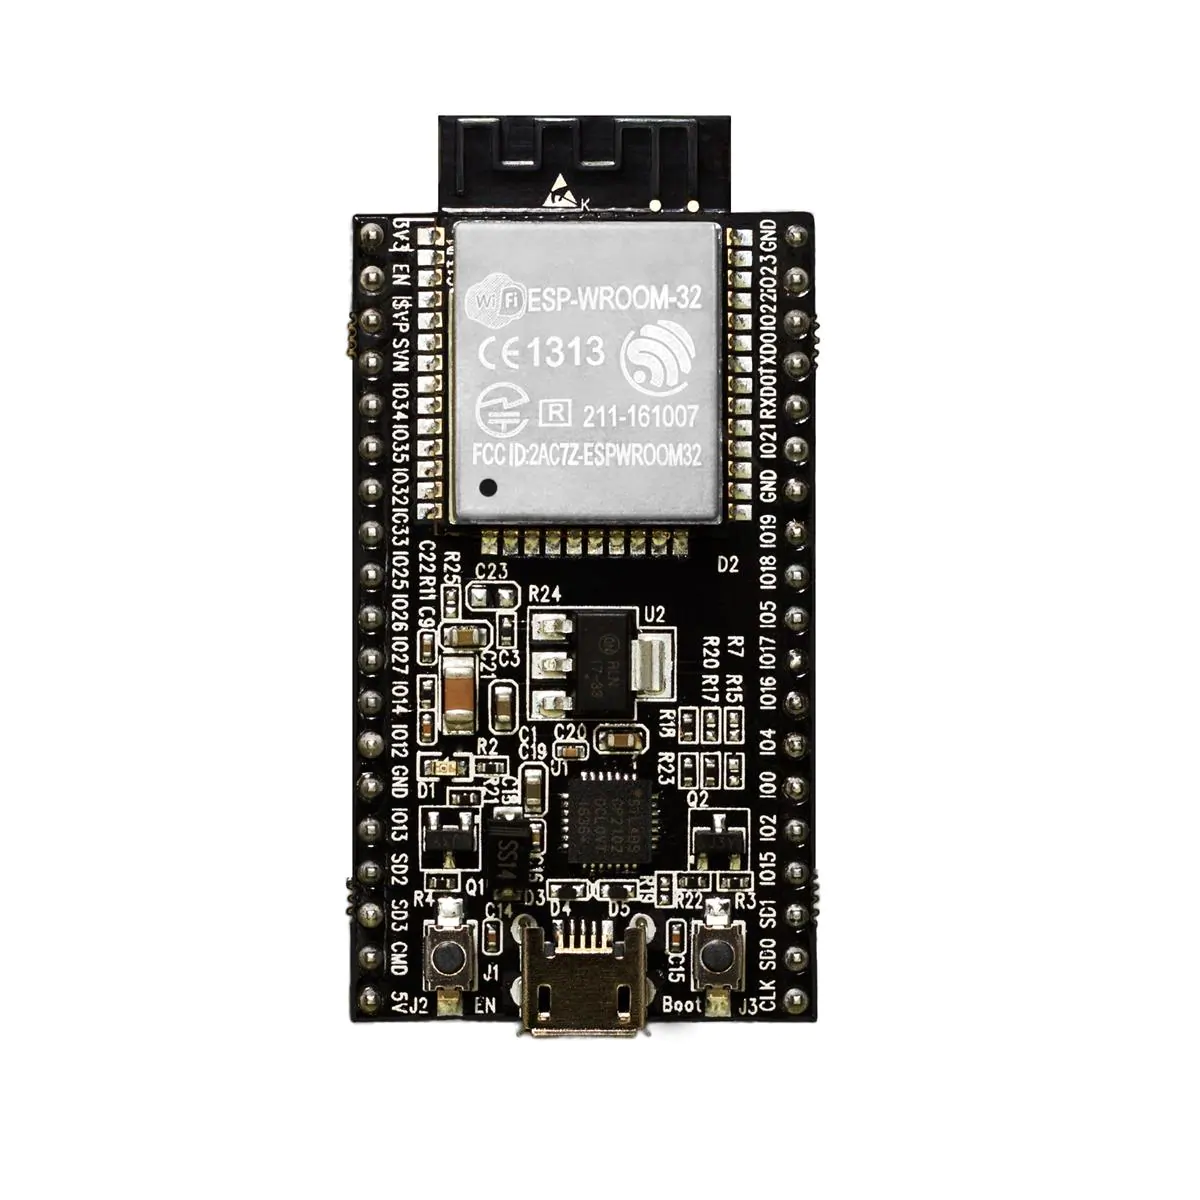
\includegraphics[scale=0.2]{analisis/esp32_devkitc_32u}
\caption{Módulo de desarrollo ESP32-DevKitC-32D}
\label{fig:esp32_devkitc_32d}
\end{figure}

\subsubsection{Framework}

Actualmente existen multitud de \textit{frameworks} de desarrollo para el SoC ESP32, basados en una gran variedad de lenguajes como: C, C++, Python, JavaScript o Lua. A continuación se analizan algunos de los  \textit{frameworks} más usados.\\

\paragraph{Espressif IoT Development Framework (ESP-IDF)}\mbox{}\\
ESP-IDF es el \textit{framework} de desarrollo oficial creado por Espressif Systems para el SoC ESP32. Está escrito principalmente en C  y está basado en el sistema operativo en tiempo real FreeRTOS. Es uno de los más usados y tiene una gran comunidad siendo fácil encontrar ayuda en sus foros oficiales, además cuenta con una extensa documentación oficial. La mayoría de \textit{frameworks} que trabajan sobre C o C++ están construidos sobre la API de ESP-IDF. Para trabajar con el solo es necesaria la \textit{toolchain} propia, algunas herramientas de construcción (CMake y Ninja) y por supuesto el propio paquete ESP-IDF que contiene la API y algunos scripts para facilitar el uso de la \textit{toolchain}. Con estas herramientas y un simple editor de texto ya podríamos empezar a crear aplicaciones para el ESP32 aunque es recomendable utilizar algún IDE como PlatformIO IDE.\\

 Las principales ventajas de este \textit{framework} es que al ser el oficial del fabricante es en el que primero obtendremos nuevas funcionalidades y parches de seguridad, otra de sus ventajas es que al tener un menor nivel de abstracción que permite un acceso a más bajo nivel que el resto, esto a su vez es su desventaja ya resulta en un código más extenso y difícil de mantener.

\paragraph{Arduino}\mbox{}\\
Arduino es una plataforma de código abierto utilizada para la construcción de proyectos de electrónica, dentro de está plataforma encontramos el lenguaje de programación Arduino y el entorno de desarrollo Arduino IDE. Arduino es un lenguaje potente y sencillo que permite desarrollar proyectos en C/C++ sin requerir grandes conocimientos de electrónica. Gracias a su espíritu de código abierto ha crecido una gran comunidad a su alrededor que ha contribuido creando todo tipo de librerías y herramientas.\\

Este lenguaje fue inicialmente diseñado para utilizarse sobre las placas Arduino pero con su creciente popularidad se han realizado multitud de adaptaciones para usarlo en otros microcontroladores como es el caso del ESP32, esta adaptación esta basada en ESP-IDF y fue realizada por el propio fabricante del SoC Espressif Systems, permite un mayor nivel de abstracción y acceso a una gran cantidad de librerías sin perder acceso a funcionalidades a más bajo nivel usando funciones del ESP-IDF ya que las librerías están integradas en la compilación de la librería de Arduino.\\

Resumiendo, sus principales ventajas son el nivel de abstracción y su comunidad, otra de sus ventajas es el entorno de desarrollo Arduino IDE que permite realizar de forma sencilla acciones como compilar o subir el código a la placa, también posible utilizarlo con el IDE de PlatformIO, ambos disponen de un gestor de librerías que permite buscar e instalarlas fácilmente. Como desventaja el tener un mayor nivel de abstracción siempre implica perder algo de control.\\

\paragraph{MicroPython}\mbox{}\\
MicroPython es una implementación del lenguaje de programación Python 3 que incluye una pequeño subconjunto de la biblioteca estándar de Python y está optimizada para ejecutarse en microcontroladores. Originalmente fue diseñado para ejecutarse sobre la placa PyBoard pero actualmente se ha adaptado a un amplio número de arquitecturas. No dispone de un IDE propio pero hay varias alternativas como uPyCraft, Thonny o  VSCode con la extensión PyMark.\\

Su principal ventaja además de portar la simplicidad del lenguaje Python al mundo de los microcontroladores es que una vez cargado en la placa podemos ejecutar comandos en el ESP32 directamente a través del serial como si fuera una consola Python normal y corriente, esto agiliza mucho el proceso de desarrollo ya que permite realizar pruebas sin tiempos de compilación ni de subida a la placa. Su mayor desventaja es que no permite acceder  a funciones a bajo nivel por ejemplo para las funcionalidades WiFi y no dispone de tantas librerías como las anteriores opciones.\\

\paragraph{NodeMCU}\mbox{}\\
NodeMCU es una plataforma de código abierto que incluye tanto el firmware basado en LUA como un módulo de desarrollo homónimo basado en los SoCs de Espressif, el lenguaje inicialmente se desarrolló para las placas NodeMCU pero ahora se puede ejecutar en cualquier módulo ESP.\\

Su principal característica es que usa un modelo de programación similar a Node.js basado en la  asincronía  y en arquitectura dirigida por eventos, la mayoría de sus funciones tienen un parámetro para funciones \textit{callback}. Como desventaja LUA no es un lenguaje muy popular por lo que normalmente requerirá que el desarrollador tenga que aprender un nuevo lenguaje desde cero, además no dispone de un IDE por lo que empezar a trabajar con el no es tan sencillo como en el resto de opciones.\\

\paragraph{Mongoose OS}\mbox{}\\
Mongoose OS es una plataforma de desarrollo de código abierto enfocada a la integración con las plataformas cloud IoT como Amazon, Azureo Google, también dispone de una versión empresarial con licencia comercial que dispone de más funcionalidades la versión libre. Su propósito es ser un entorno completo para la creación de prototipos, desarrollo y gestión de dispositivos conectados.\\

Una de sus principales ventajas es que permite programar tanto en JavaScript como en C, además dispone de un IDE muy completo con interfaz web. Su principal desventaja es que algunas librerías son de código cerrado y es necesario adquirir una licencia para poder utilizarlas. También cabe destacar que aunque la opción de programar con JS pueda resultar atractiva para un prototipado rápido durante el desarrollo no es recomendable usarlo en producción ya que tiene una mayor sobrecarga en consumo de memoria y CPU.\\

\paragraph{Elección}\mbox{}\\

Tras analizar los \textit{frameworks} expuestos anteriormente se optó por elegir Arduino como solución para este proyecto, las razones para esta elección han sido su gran facilidad de uso y sencillez como se puede ver en el Código \ref{lst:arduino_example}, dispone de una gran comunidad y trayectoria por lo que es muy fácil encontrar información y respuestas a cualquier duda, dispone de una gran cantidad de librerías que facilitaran el trabajo y además a pesar de su gran nivel de abstracción podemos seguir accediendo a bajo nivel gracias a la integración con ESP-IDF, requisito necesario en este proyecto dada la necesidad de utilizar las funciones de monitorización del tráfico WiFi no disponibles en la mayoría de \textit{frameworks}.\\

\begin{minipage}{\linewidth}
\begin{lstlisting}[language=C, caption=Ejemplo de código para hacer parpadear un led con Arduino, captionpos=b, frame=single, label={lst:arduino_example}]
const int LED_BUILTIN = 2;

void setup() {
  pinMode (LED_BUILTIN, OUTPUT);
}

void loop() {
  digitalWrite(LED_BUILTIN, HIGH);
  delay(1000);
  digitalWrite(LED_BUILTIN, LOW);
  delay(1000);
}
\end{lstlisting}
\end{minipage}

\subsection{Servidor central}

En esta sección se describirán las herramientas elegidas para el desarrollo del servidor central encargado de recibir y almacenar las detecciones de los sensores a través de una API REST y de mostrar estas detecciones de una forma amigable a través de una interfaz web o a través de la propia API. Para ello has sido necesario seleccionar un \textit{framework} web que nos permita desarrollar la aplicación web y una base de datos que nos provea de persistencia para almacenar las detecciones.

\subsubsection{Framework web}

En la actualidad existen muchas opciones para crear aplicaciones web en multitud de lenguajes de programación, algunos de los más conocido son Ruby on Rails (Ruby), Laravel (PHP), Spring (Java) y Django (Python). En la búsqueda de esta herramienta el principal requisito que se buscaba era la posibilidad de desarrollar en algún lenguaje ya conocido de forma que la curva de aprendizaje fuera menor y permitiera un desarrollo más rápido, ademas se planteaban otros requisitos deseables:

\begin{itemize}
  \item Simplicidad.
  \item Ligero.
  \item Facilidad para desarrollo de API REST.
  \item Agnóstico respecto a la base de datos a utilizar.
  \item Compatible con modelo MVC.
  \item Facilidad para su despliegue mediante contenedores.
  \item Buena documentación y madurez en el mercado.
\end{itemize}

El principal requisito condujo a analizar los principales entornos de desarrollo para Python, estos son Django y Flask, ambos tienen una gran trayectoria y una gran comunidad detrás, además el haber trabajado anteriormente con ellos proporciona una visión más detallada de su funcionamiento, ventajas y desventajas.\\

Django es con diferencia el \textit{framework} basado en Python más popular. Está enfocado a la creación de aplicaciones web complejas basándose en el patrón de diseño MVC, sigue la filosofía de \textquote{baterías incluidas}, esto quiere decir que intenta proveer todas las herramientas que puedan ser necesarias \textquote{de fábrica}, para ello incluye una gran cantidad de herramientas como una potente interfaz de administración, su propio lenguaje de plantillas y un sistema de autenticación de usuarios. Provee una interfaz para interactuar con las bases de datos aunque su compatibilidad es limitada (PostgreSQL, MariaDB, MySQL, Oracle y SQLite).\\

Flask es un \textit{microframework} web escrito en Python que permite crear aplicaciones web de una forma rápida y sencilla. La denominación de \textit{microframework} se debe a su baja dependencia de librerías externas, de base sus únicas dependencias son la librería de utilidades WSGI Werkzeug y el motor de plantillas Jinja 2. Pero a pesar de su sencillez nos permite escalar hacia aplicaciones más complejas con la adición de extensiones que nos permiten añadir nuevas funcionalidades, por ejemplo, flask-Sqlalchemy para generar modelos de datos o flask-WTF para generar formularios. Este tipo de diseño nos proporciona un entorno de desarrollo muy ligero y al haber poca dependencia minimiza el trabajo de actualización y control de errores de seguridad ya que solo utilizaremos las extensiones que realmente necesitamos, a diferencia de otros \textit{frameworks} como Django que incluyen utilidades que probablemente no lleguemos a utilizar.\\

Tras analizar estas dos opciones la solución elegida ha sido el \textit{microframework} Flask principalmente por su facilidad y simplicidad ya que lo convierten en una solución ideal para aplicaciones web pequeñas como es el caso de este proyecto, también nos permite una mayor flexibilidad en el diseño mediante el uso de extensiones, además permite crear APIs de una forma más sencilla y con menos código. Otra ventaja sobre Django es que gracias a su diseño minimalista en líneas generales tiene un mejor rendimiento en tiempos de respuesta, algo fundamental en un proyecto como este en el que se realizarían una gran cantidad de peticiones. Otras características que han propiciado esta elección son las siguientes:

\begin{itemize}
  \item Servidor de desarrollo integrado y depurador.
  \item Soporte integrado para pruebas unitarias.
  \item Motor de plantilla Jinja 2.
  \item Basado en Unicode.
  \item Agnóstico respecto a la base de datos.
  \item Compatible con WSGI.
  \item Documentación extensa.
\end{itemize}

En el siguiente código podemos ver un ejemplo de su sencillez, con menos de diez lineas de código podemos desplegar una sencilla aplicación web que nos devuelve el clásico \textit{Hello, World!}\\

\begin{minipage}{\linewidth}
\begin{lstlisting}[language=Python, caption=Ejemplo de aplicación web básica con Flask, captionpos=b, frame=single]
from flask import Flask
app = Flask(__name__)

@app.route("/")
def hello():
    return "Hello World!"

if __name__ == "__main__":
    app.run(debug=True)
\end{lstlisting}
\end{minipage}

\subsubsection{Base de datos}

 Una vez definida la solución a utilizar para recolectar las detecciones es necesario definir como almacenaremos estas detecciones y para ello utilizaremos una base de datos. Cabe destacar que tal y como se indicó en los objetivos no es propósito de este proyecto el posterior procesamiento de estos datos, por tanto en la elección de esta solución no se tendrá tanto en cuenta el rendimiento en la lectura y agregación de los datos como el rendimiento de escritura y la simplicidad en la implementación e integración de la solución.\\

En este análisis se tuvieron en cuenta tanto bases de datos tradicionales SQL como NoSQL. Estas últimas cuentan con gran popularidad en el mercado IoT debido a su gran versatilidad ya que no requieren estructuras fijas como tablas si no que suelen utilizar sistemas de almacenamiento basados en estructuras de clave-valor o en forma de documentos, es decir, cada registro puede contener una información con diferente forma de otro registro dentro del mismo conjunto, otra de sus ventajas es que son altamente escalables horizontalmente. Como principales desventajas no suelen permitir operaciones \textit{JOIN} ni garantizan las características ACID (atomicidad, consistencia, aislamiento y durabilidad). Algunos ejemplos de este tipo de tecnología son MongoDB, CouchDB o Cassandra.\\

Los sistemas de base de datos NoSQL presentan grandes ventajas para sistemas IoT no homogeneizados dada su gran dinamicidad en la ingesta de los datos, pero esta característica no será necesaria en este proyecto ya que la información que se almacenará será estable y bien definida su estructura desde el inicio del proyecto. Tampoco se observan grandes diferencias de rendimiento respecto a los sistemas tradicionales, siendo estos últimos incluso más eficientes en la inserción \cite{ASIMINIDIS2018} \cite{RAUTMARE2016} que como se ha mencionado anteriormente primará en los requisitos respecto al rendimiento en lectura.\\

Estos motivos junto a la familiaridad con los sistemas tradicionales SQL, su gran ecosistema y madurez en el mercado han llevado a seleccionar como solución el sistema de gestión de base de datos relacional PostgreSQL.

\subsubsection{Herramientas de despliegue}

Para el despliegue del servidor web y de la base de datos se ha decidido utilizar contenedores, tanto en la etapa de desarrollo como en la puesta en producción. En general, las ventajas que ofrece un entorno de despliegue de aplicaciones sobre contenedores son las siguientes:\\

\begin{itemize}
  \item Ligereza: Respecto a soluciones tradicionales como máquinas virtuales son mucho más ligeras en tamaño y en consumo ya que no inician una copia completa del sistema operativo.
  \item Escalado: Debido a su ligereza el arranque de los contenedores es muy rápido en comparación a los sistemas tradicionales, podemos desplegar nuevas réplicas en unos segundo si la demanda sube y volverlas a destruir cuando ya no son necesarias.
  \item Estandarización de los despliegues: Las aplicaciones que se ejecutan sobre un contenedor están aisladas del resto del sistema y por lo tanto los contenedores se pueden migrar fácilmente de una máquina a otra sin preocuparse por problemas de compatibilidad.
  \item Facilidad para aplicar parches y actualizaciones: Los contenedores se basan en imágenes inmutables, por lo que para aplicar un parche simplemente se genera una imagen nueva y se cambia la configuración del servicio para usarla.
  \item Independencia de la infraestructura subyacente: No importa si los hosts sobre los que se despliegue este tipo de plataforma son servidores físicos, máquinas virtuales en un CPD local, o servidores virtuales de algún proveedor como Amazon, Microsoft o Google, una vez estén configuradas, las aplicaciones desplegadas en ella van a funcionar sin apenas ningún cambio en cualquiera de esas situaciones.
  \item Mayor consistencia entre los entornos de prueba: Toda la definición de la imagen sobre la que se ejecutará nuestra aplicación está descrita en un fichero por lo que no harbá prácticamente diferencias entre los entornos.
\end{itemize}

La tecnología seleccionada para la creación de los contenedores ha sido Docker, es sin lugar a dudas la herramienta de contenedores más popular y utilizada, por lo que disponemos de mucha información y ayuda.\\

Para orquestar el despliegue de estos contenedores también se utilizará la herramienta Docker Compose, esta herramienta nos permite definir mediante un fichero YAML como se desplegaran los contenedores, facilitando herramientas para la carga de variables de entorno, exponer puertos o definir dependencias entre los contenedores.\\

Una vez seleccionada la solución para desplegar las aplicaciones queda definir sobre que infraestructura se desplegará, para la fase de desarrollo se ha optado por desplegar en mi propio equipo utilizando solamente las herramientas mencionadas, sin embargo para un entorno de producción necesitamos un entorno con alta disponibilidad, escalabilidad y con facilidad de acceso externo. Para responder a estas necesidades se ha decidido utilizar una plataforma como servicio, denominado PaaS por sus siglas en ingles (\textit{Platform as a Service}), este concepto describe un tipo de servicio en la nube que nos proporciona una plataforma para desplegar aplicaciones sin la complejidad de construir y mantener nosotros la infraestructura, simplemente subiremos nuestro código y este se desplegará automáticamente. La plataforma elegida ha sido Heroku, es uno de los PaaS más utilizados en la actualidad, ofrece soporte para una gran variedad de lenguajes: Node.js, Ruby, Python, Java, PHP, Go, Scala y Clojure; bajo el capó estas aplicaciones son desplegadas mediante contenedores denominados \textit{dynos}, además nos ofrece la posibilidad de instalar \textit{addons} para agregar funcionalidades a estos contenedores, por ejemplo, servicios de base de datos, monitorización y \textit{logging}.\\

 Esta plataforma se distingue por su sencillez, nos permite desplegar una nueva aplicación en cuestión de minutos, por ejemplo, para una aplicación Python solo necesitamos crear un nuevo proyecto a través de su interfaz web o de su cliente de CLI, una vez creado nos proporcionará un enlace a un repositorio Git dónde podremos subir el código y se desplegará automáticamente, lo único que necesitaremos hacer antes de subirlo es disponer del clásico archivo \textit{requirements.txt} con las dependencias de nuestra aplicación Python en el raíz del repositorio y un simple fichero llamado \textit{Procfile} dónde especificaremos como debe arrancarse nuestra aplicación.\\

 \begin{minipage}{\linewidth}
 \begin{lstlisting}[caption=Ejemplo de fichero Procfile para desplegar una aplicación Flask en Heroku , captionpos=b, frame=single]
 web: gunicorn app:app
 \end{lstlisting}
 \end{minipage}

\end{document}
